% --------------------------------------------------------------------------- %
\chapter{Measurements and Data Processing}
\label{chap:measurementProcess}
% --------------------------------------------------------------------------- %

\todo[inline]{%
    Primary questions to answer in this chapter: What did we measure, how, and
    why?
}

This chapter elaborates  on what measurements were performed  and what special
considerations, if any,  had to be taken into  account. Additionally, the work
flow for the processing of the obtained data is explained.


% --------------------------------------------------------------------------- %
\section{Measurements}
\label{sec:measurements}
% --------------------------------------------------------------------------- %

In total,  ten chips have been  evaluated. While this number is  far below the
\num{1027} samples  which would be  needed to  obtain a range  which contains,
with a probability as low as \SI{75}{\percent}, all but \SI{0.27}{\percent} of
the chips coming from the same manufacturing batch (see \cite{ref:3sfall}), it
does  give at  least some  additional  statistical confidence  in our  results
beyond measuring simply a single sample.

The measurements were  conducted for a range of DC  input signals. This allows
to to assess linearity, correctness of gain, offset and time constants for the
pre-amplifier.

The  differential amplifier  outputs  a signal  which  oscillates between  the
reference  voltage  (\SI{1.5}{\volt}) and  the  difference  between the  input
voltage  and the  reference voltage,  multiplied by  the signed  gain, as  per
equation \ref{eq:vdiff}:

\begin{equation}
    \label{eq:vdiff}
    V_{\mathrm{out, preamp}} = ( V_{\mathrm{in}} - \SI{1.5}{\volt} ) \cdot \mathrm{Gain}
\end{equation}

Below  \SI{0.5}{\volt}  and  above  \SI{2.5}{\volt},  the  circuit  goes  into
saturation,  so  keeping  $V_{\mathrm{out,  preamp}}$  inside  that  range  is
desired. Consequently, the range  of sensible input voltages  changes with the
gain. Table \ref{tab:measurementSuite}  presents an excerpt of  the test suite
as  it was  performed on  the  pre-amplifier of  a  single chip  for a  single
sampling frequency and positive gains.

\begin{table}
    \centering
    \caption{%
            Measurement  suite  for  a  single  chip  for  the  pre-amplifier,
            with    positive    gain    and   a    sampling    frequency    of
            \SI{32}{\kilo\hertz}. This was  repeated for  sampling frequencies
            \SI{96}{\kilo\hertz} and  \SI{256}{\kilo\hertz}, respectively, for
            negative gains of identical magnitude,  for the \sdm~ and for both
            elements,  for nine  more chips,  resulting in  roughly \num{4000}
            measurements.%
        }
    \label{tab:measurementSuite}
    \scriptsize
    \rowcolors{2}{solarized-base3}{white}
    \begin{tabular}{rrrr}
        \toprule
        \textsc{Gain} & \textsc{Input Voltage} & \textsc{Element Measured} \\
        \midrule
        +1 & \SI{0.5}{\volt} & Preamp \\
        +1 & \SI{0.7}{\volt} & Preamp \\
        +1 & \SI{0.9}{\volt} & Preamp \\
        +1 & \SI{1.1}{\volt} & Preamp \\
        +1 & \SI{1.3}{\volt} & Preamp \\
        +1 & \SI{1.5}{\volt} & Preamp \\
        +1 & \SI{1.7}{\volt} & Preamp \\
        +1 & \SI{1.9}{\volt} & Preamp \\
        +1 & \SI{2.1}{\volt} & Preamp \\
        +1 & \SI{2.3}{\volt} & Preamp \\
        +1 & \SI{2.5}{\volt} & Preamp \\
        \midrule
        +2 & \SI{1.0}{\volt} & Preamp \\
        +2 & \SI{1.1}{\volt} & Preamp \\
        +2 & \SI{1.2}{\volt} & Preamp \\
        +2 & \SI{1.3}{\volt} & Preamp \\
        +2 & \SI{1.4}{\volt} & Preamp \\
        +2 & \SI{1.5}{\volt} & Preamp \\
        +2 & \SI{1.6}{\volt} & Preamp \\
        +2 & \SI{1.7}{\volt} & Preamp \\
        +2 & \SI{1.8}{\volt} & Preamp \\
        +2 & \SI{1.9}{\volt} & Preamp \\
        +2 & \SI{2.0}{\volt} & Preamp \\
        \midrule
        +4 & \SI{1.25}{\volt} & Preamp \\
        +4 & \SI{1.30}{\volt} & Preamp \\
        +4 & \SI{1.35}{\volt} & Preamp \\
        +4 & \SI{1.40}{\volt} & Preamp \\
        +4 & \SI{1.45}{\volt} & Preamp \\
        +4 & \SI{1.50}{\volt} & Preamp \\
        +4 & \SI{1.55}{\volt} & Preamp \\
        +4 & \SI{1.60}{\volt} & Preamp \\
        +4 & \SI{1.65}{\volt} & Preamp \\
        +4 & \SI{1.70}{\volt} & Preamp \\
        +4 & \SI{1.75}{\volt} & Preamp \\
        \midrule
        +8 & \SI{1.375}{\volt} & Preamp \\
        +8 & \SI{1.425}{\volt} & Preamp \\
        +8 & \SI{1.475}{\volt} & Preamp \\
        +8 & \SI{1.500}{\volt} & Preamp \\
        +8 & \SI{1.525}{\volt} & Preamp \\
        +8 & \SI{1.575}{\volt} & Preamp \\
        +8 & \SI{1.625}{\volt} & Preamp \\
        \midrule
        +16 & \SI{1.450}{\volt} & Preamp \\
        +16 & \SI{1.475}{\volt} & Preamp \\
        +16 & \SI{1.500}{\volt} & Preamp \\
        +16 & \SI{1.525}{\volt} & Preamp \\
        +16 & \SI{1.550}{\volt} & Preamp \\
        \bottomrule
    \end{tabular}
\end{table}

The process of performing the measurements  is based on the scripts documented
in the previous chapter.


% --------------------------------------------------------------------------- %
\section{Data Processing}
\label{sec:dataProcessing}
% --------------------------------------------------------------------------- %


The goal in this project was  to create an efficient, streamlined workflow for
measuring  multiple sensor  chips and  correlating the  results in  meaningful
ways.   The  conclusions  drawn  in  this report  mostly  originated  from  DC
measurements; A number  of known voltages are applied to  the chip's input and
its output  is observed. There  are multiple configurations  to do  this with,
namely in function  of the preamp gain and the  sampling frequency $fs$, which
in turn can be done again as a whole for just the preamp, for just the \sdm~or
for both  combined (the whole  chip). These measurements were performed  on 10
different chips that  all originated from the same wafer.   This gives us some
statistical  reinforcement in  the results,  assuming the  whole wafer  is not
biased of course.

\begin{figure}[t]
    \centering
    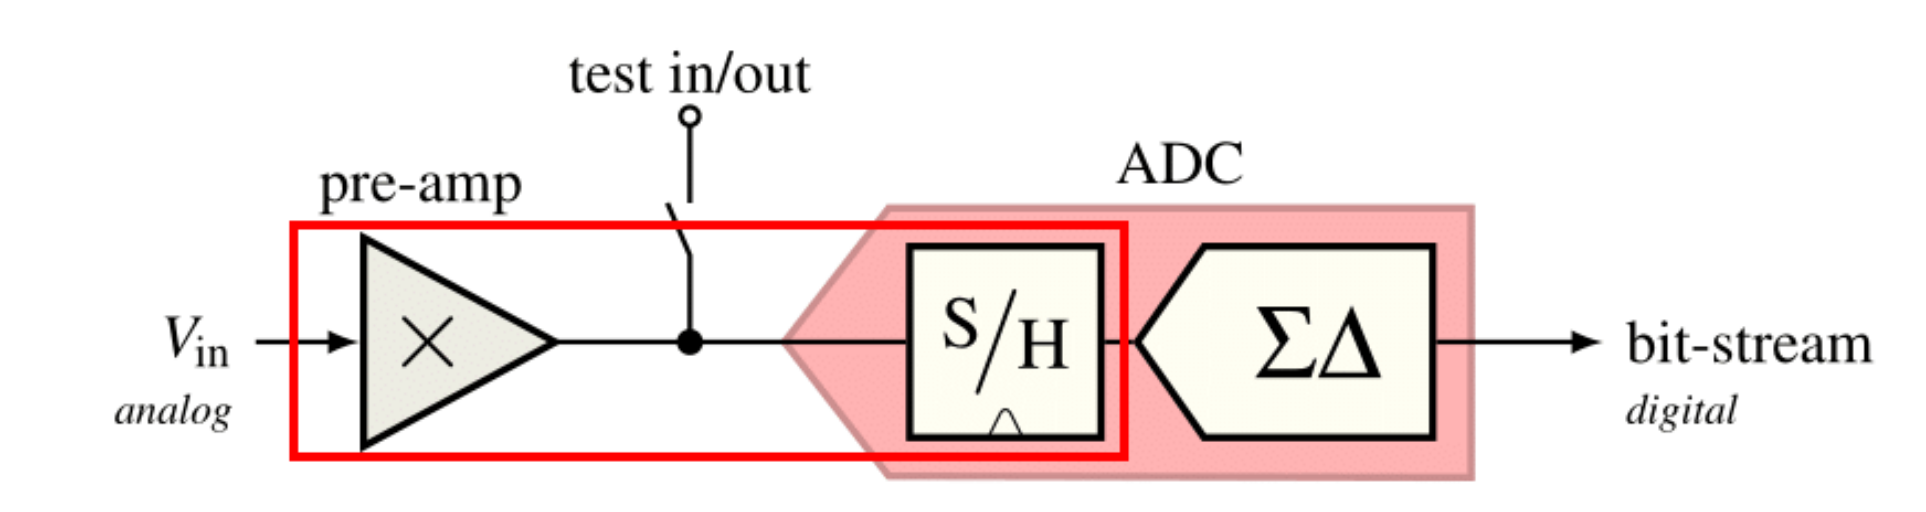
\includegraphics[width=.8\linewidth]{images/blockdiagram.png}
    \caption{Rough block diagram of the sensor chip}
    \label{fig:blockdiagram}
\end{figure}

Figure \ref{fig:blockdiagram} shows a rough overview of the chip's components.

The preamp is responsible for amplifying the difference of an input voltage to
a  $\SI{1.5}{\volt}$ reference voltage by an  externally  configurable  factor
(either  by  1,  2,  4,  8,  or 16). Additionally, the amplifier can be set to
invert the gain.

The SAH  (Sample and Hold) block  works together with the  \sdm~to convert the
analog voltage from the preamp into a digital bit-stream.

There are two different  kinds  of measurements which had to be performed: The
output from measurements involving the \sdm~were recorded using  a GPIO pin on
a  \raspi.  Here,  the  input  signal  is  either  applied to the preamp (when
measuring the whole  device)  or  to the \signal{TEST OUT} pin (when measuring
the \sdm~alone). The output from the preamp on the other hand is analog, so it
needed to  be  measured  using  an oscilloscope via the \signal{TEST OUT} pin.

For both the preamp as well as the \sdm, DC measurements over an input voltage
range   between   \SI{0.5}{\volt}  and  \SI{2.5}{\volt}  were  performed.   AC
measurements  are  used   to   assess   the   system's   frequency   behavior.

The sample size is 10 chips, unless indicated otherwise.

Based on these  measurements and their analysis in the next chapter, we strive
to answer the question of what sort of use cases this system  is suitable for,
and with which settings.

% TODO: noise
% TODO: resolution in bits under a given set of circumstances
% TODO: Measurement methodology


% --------------------------------------------------------------------------- %
\section{Pre-Amplifier: DC Measurements}
\label{sec:preAmpDC}
% --------------------------------------------------------------------------- %



% --------------------------------------------------------------------------- %
\section{Sigma-Delta Converter: DC Measurements}
\label{sec:sigdelDC}
% --------------------------------------------------------------------------- %

% --------------------------------------------------------------------------- %
\section{Complete System: DC Measurements}
\label{sec:systemDC}
% --------------------------------------------------------------------------- %

